% A wedge sum X ∨ Y depicted as a square with a circle attached, equal to the
% square wedged with the circle.
% Source: book/tex/homology/cup-product.tex (§ Wedge sums).
\documentclass[border=2mm]{standalone}
\usepackage{tikz}
\begin{document}
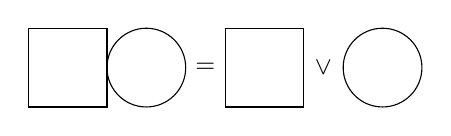
\begin{tikzpicture}[scale=1, every node/.style={font=\small}]
  % X ∨ Y : unit square with a small circle attached
  \draw (-1,0) rectangle (0,1);
  \draw (0.5,0.5) circle (0.5);
  \node at (1.25,0.5) {$=$};
  % the square factor
  \draw (1.5,0) rectangle (2.5,1);
  \node at (2.75,0.5) {$\vee$};
  % the circle factor
  \draw (3.5,0.5) circle (0.5);
\end{tikzpicture}
\end{document}
